\documentclass[12pt]{ruthesis}
\usepackage{amsmath}
\usepackage{amssymb}
\usepackage{latexsym}
\usepackage{graphics}
\usepackage{epsfig,epsf,rotating}
%\usepackage{adjustbox}      
\usepackage{subfigure}
\usepackage{graphicx}
%\usepackage{pictex}
\usepackage{epsf}
%\usepackage{cite}
\usepackage{theorem}
\usepackage{verbatim}
\usepackage{float}
\usepackage{xcolor}
\usepackage{appendix}
\usepackage{inputenc}
%%%
\usepackage{adjustbox}
%%%

%\usepackage[table,xcdraw]{xcolor}

\newtheorem{proposition}{Proposition}

\theoremheaderfont{\itshape} {\theoremstyle{break}
\newtheorem{Fact}{Fact}[chapter]} \theoremstyle{break}
\newtheorem{Lem}{Lemma}[chapter] \theoremstyle{break}
\newtheorem{Thm}{Theorem}[chapter] {\theoremstyle{plain}
  \theorembodyfont{\rmfamily}  \newtheorem{Prf}{Proof}[chapter]}
{\theoremstyle{plain}
  \theorembodyfont{\rmfamily}  \newtheorem{Def}{Definition}[chapter]}

\title{Using Multiple Imputation, Survival Analysis, 
And Propensity Score Analysis In Cancer Data With Missingness}
%I have no idea what ctitle does
%\ctitle{Put a cool title herefdfdfd}
\author{Nathan Karmazin Berliner}
\department{Statistics}
\school{Rice University}
\degree{Master of Arts \\Statistics}

\committee {
        Rudy Guerra, Committee Chair \\
        Professor of Statistics \and
        Kenneth Hess, Thesis Director \\
        Professor, MD Anderson Cancer Center\and
        Yu Shen\\
        Professor, MD Anderson Cancer Center \and
        Marina Vannucci\\
        Professor of Statistics \and
        David Scott\\
        Professor of Statistics
}


\address{Houston, Texas}
\donemonth{December} \doneyear{2015} \makeindex
\begin{document}

  \begin{frontmatter}
   \pagenumbering{roman}
   %\makecover
   \maketitle
   \thispagestyle{empty}
\begin{abstract}
I will write my abstract here.
\end{abstract}



   %figure out the ack later
   %\section*{Acknowledgements}
\thispagestyle{empty}

I would like to thank my family, friends, and professors for getting me through all of this!

   %\include{ack}
   \tableofcontents
   \listoffigures
   \listoftables
   %\include{ded}
  \end{frontmatter}
\pagenumbering{arabic}

\linespacing{1.7}

\chapter{Introduction and Background Information}
\section{Motivation}
\label{sec:Motivation}
The motivation of this thesis is to show the methodology that can be used both by applied researchers and clinicians to draw meaningful survival and causal inference from imputed data. While all three fields (imputation, survival, causal)  are well studied, their interaction is not. I want the methods to be easy enough to describe to someone with a limited statistical background, but meaningful and valid so that the results obtained can be used in publication. The desire to have it this way stems from working on a related project with both statisticians and clinicians. While this thesis is motivated by cancer data, I believe that the methods used in this thesis are general enough to be applied to other types of data and situations.

\label{ch:Intro}
Missing data is a major problem in both statistics and medicine; however, it has not received attention proportional to its need. Survival analysis is well studied, but is relatively complete, so little new research comes out of this field. Propensity score analysis will help us determine causal relationships when we don't have a randomized controlled experiment. As one could imagine, all three of these fields are important to the applied statistician, as they will come across at least one at some point in their career.  The goal of this thesis is to demonstrate how to use all three in trio, a topic that has only received little interest in the literature. I will explain each of these three disciplines in detail before we dive into combining them.

\section{Imputation}
\label{sec:Imputation}
In an ideal world, we would have complete data with no missingness, however this is rarely ever the case. Imputation (specifically multiple imputation) is a way to ``fill in missing data'' with plausible values, and it forms the base of this thesis. All of the other analyses that will be used will follow from it, thus we need a solid understanding of it before we may proceed. Imputation itself has been around since the 1930's \cite{VanBuuren2012}, but multiple imputation is a recent development, proposed in the 1970's and formalized in 1987 by Donald Rubin \cite{Rubin1987}. To understand the use and importance of multiple imputation, we need to understand the problem of missing data, and the previous attempts to deal with it.

At first, statisticians paid no attention to missing data, and happily discarded records from their data that were incomplete. This procedure is known as complete case (CC) analysis. There are many problems with this paradigm. To begin with, you will lose a lot of statistical power when, because you are throwing away records and thus decreasing your sample size. In addition, this can be costly to the researcher. If it costs a set amount to collect a single record, and you don't use this record, you are wasting money. As well, in some rare cases, incomplete data might be the only type we can get (e.g. if we have a machine that analyzes a blood sample chemical level, but can't detect it if the level is too high or low). Lastly, and most importantly, we will be biasing our estimates if we discard them. For example, suppose we have a random sample of people and are testing a drug�s efficacy, and want to run a regression on some collected covariates. If men are known to not want to give all of their information, in the analysis, we will need to discard the male samples because they are incomplete, leaving us only with women. Thus, we no longer have a random sample, and will get biased results because we have knowingly thrown away half of our data which we know to be different \cite{VanBuuren2012}.

A slight improvement on this is called available case (AC) analysis. In this setting, a record is used in the analysis if it has all of the needed information for that analysis. So, a record could have missingness, but if the covariate with missingness is never used in the analysis, it will not be discarded. This paradigm is the standard analysis type for most statistical packages. It is better than complete case analysis, but is still flawed. We are still throwing away valuable data as we were with complete case analysis, although likely not as much. Available case analysis will still lead to bias in the same way that complete case did too. As well, new complications arise in available case analysis, namely that nonsensical situations like correlations outside of $\pm 1$, and inconsistent sample sizes for different analyses can arise.

The next wave of statisticians in the early $20^{th}$ century wanted to improve upon available case analysis, so they developed what we now call today imputation. Their specific incarnation was called single imputation, and their goal was to fill in missing values with a single plausible replacement value. A single method (such as regression, taking the mean, resampling) is used one time to impute or fill in the missing value. While this is a little better than complete case analysis, it still has many drawbacks. Asserting that a single value is the true value is unjustified. There is always some amount of error and uncertainty involved, and we can in no way be 100\% confident that our imputed value is correct. Furthermore, if I impute one value and you impute another, we may get completely different results from analysis on the data. This is obviously not a desirable trait.  In addition, imputing one time and calling it your true data will artificially increase your sample size. You are in effect treating the imputed values as if they were real, inflating your sample size with data that was not actually observed. This will give you unjustified statistical power and accuracy. While single imputation certainly has its drawbacks, the idea of actually trying to fill in the data is an important one, and multiple imputation fills in the gaps that single imputation is not able to cover.

Multiple imputation (MI) began in the 1970's, but it wasn't until 1987 when Donald Rubin formalized multiple imputation methodology in his seminal book \emph{ Multiple Imputation for Nonresponse in Surveys} did it start to gain acceptance \cite{Rubin1987}. The central idea is to frame the problem in a Bayesian framework, and produce $m\geq 2$ values to substitute in for each missing value, drawing these values from the missing covariates posterior distribution. Using these substitute values ($m$ values), we can think of the data now as being m datasets, each dataset containing the observed data, and one value for each piece of missing data. 

An example will make the MI process clear. Suppose that we had a dataset of age, weight, and height. We want to regress age on weight but we have missingness. First, we will impute our data (figure \ref{fig:miexample}, the first two columns). Once we have a sufficient number of datasets (we will talk about how to pick the number later), we can run out analyses on each of the MI datasets, treating the dataset as if it was complete (horizontal lines and third column). After running the model on the $m$ datasets, we can pool the results to get one single estimate with its associated variance (last column).  
\begin{figure}[!ht]
  \centering
    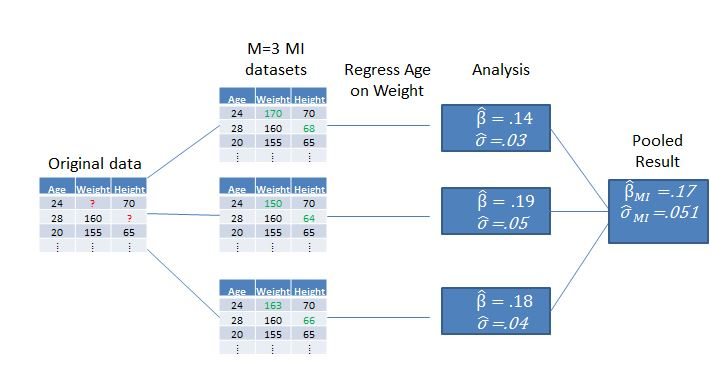
\includegraphics[width=0.8\textwidth]{mi_example_full.jpg}
  \caption{Visualization of MI data}
\label{fig:miexample}
\medskip
\small
In the original data, missingness is displayed by \textcolor{red}{?'s} and the imputed data is shown in the multiply imputed data as \textcolor{green}{\#'s}. We then regress age on weight, get the results from the individual datasets, and then pool them together.
\end{figure}


This method is obviously much better than the first two methods because it allows us to not throw away data, as well as to quantify our uncertainty about imputing the missing values. The only real drawback of multiple imputation is that we still don't have true data, but we can be confident enough in our estimations to compensate for that. The only better option would be to not have any missing data.

The use of multiple imputation has been steadily increasing over the past 30 years, and it is now the standard for missing data. Stef van Burren, an influential author in multiple imputation did a study of academic papers, and concluded that the number of publications using or mentioning multiple imputation is growing at an exponential rate since about 1990 \cite{VanBuuren2012}. Thus, using multiple imputation will be advised because of its popularity and strength.



\section{Survival}
\label{sec:Survival}
Survival analysis is a huge field, and there have been many textbooks written about it. I only plan to introduce the topics that are relevant to my case study.  For a much more detailed account of survival analysis, please see \cite{Klein1984}.

Survival analysis on the whole can generally be described as the analysis of time to event data, often in the presence of censoring or truncation (when we don't have complete information about the time of event).  There are many techniques used in this field, but the main tools that we will be using are Kaplan-Meier estimates, log rank tests, and Cox regression. 

Before we go on, it should be noted that often in the literature and software (and in this paper) we see terms like ``death/failure'' and ``survivors''. This is due to survival analysis being heavily influenced and intertwined with medical studies. A more general term for these would be ``event'' and ``those who have not had an event yet''. These terms are used because they are clear and concise, although it might not accurately describe the event at hand. For example, if we were tracking the time until a child loses all of their baby teeth; the term death would obviously not portray the event of interest, but may be used in the context to denote losing all of the teeth.

The Kaplan-Meier (KM) estimator is a nonparametric estimate of the true survival function (the probability that you survive after time t, $S(t)=P(T>t)=\int_t^\infty f(u)du$, where $f(u)$ is the unknown probability density function).  It is defined as 
$$\hat{S}(t)=\prod_{t_i<t}\frac{n_i-d_i}{n_i}$$
Where $n_i$ is the risk set, defined as the number of people who have not had the event or been censored right before time $t_i$ ,and $d_i$ is the number of deaths or events that you observe at time $t_i$ \cite{Kaplan1958}. The Kaplan-Meier estimator is very commonly used as a measure to see how different treatments affect the survival of the population in question, and is helpful in seeing at what time points survival changes the most (i.e. early or late). 

The log rank test is a popular nonparametric test that researchers often use to see if two or more survival curves come from the same distribution \cite{Bland2004}. This is a useful tool to have, because visualizing curves alone does not give us this information. We could have two curves that look radically different due to sampling error, yet still come from the same distribution. Knowing if the survival curves come from the same or different distribution is useful because it allows us to make statements like ``drug A is associated with longer survival time than drug B''.

The general log rank test is defined as:
$$\frac{\sum_{j=1}^{J}w_j(O_{1j}-E_{1j})}{\sqrt{\sum_{j=1}^{j}w_j^2V_{j}}}\sim N(0,1)$$
Where $w_j$ is the weight of each individual (must be $\geq 0$, we will set all to be 1), and $N_j=N_{1j}+N_{2j}$ is the number of subjects in the risk set at time j, composed from the sum of the number of deaths at time j in each group, $O_j=O_{1j}+O_{2j}$ is the observed number of deaths at time j, composed of the sum of deaths from either group at time j,  which leads to the desired quantities $E_{1j}=\frac{O_jN_{1j}}{N_j}$ , and $V_j=\frac{O_j(N_{1j}/N_j)(1-N_{1j}/N_j)(N_j � 0_j)}{N_j -1}$

Since we set all of the weights to be 1, this test, as it is, places equal weight to all of the deaths we observe. We could change these weights though to give more emphasis to certain death times. This is useful for example if we have a drug that takes a long time to start working. We wouldn't care about early deaths, only about later times when we are comparing the survival. Putting more weight on the later deaths would help to answer this question better. It can be proven that the log rank test is equivalent to the score test on a Cox model (which will be discussed next) fit the same data with no ties \cite{Klein1984}.

Proportional hazards regression, often called Cox regression or Cox model is a modelling tool that allows us to analyze the hazard ratio of a covariate, assuming that each covariate acts to multiply the hazard ratio. 

The hazard function is a survival tool that tells us the rate of events at time $t$, conditional on survivorship until time $t$. Mathematically, it is given by:
$$\lambda(t)=\lim_{\Delta t\rightarrow 0+}\frac{P[t\leq T<t+\Delta t|t \leq T]}{\Delta t}$$.
Cox regression is a maximum (partial) likelihood method estimator, given by: 
$$h(t|Z)=h_{0}(t)\exp(\sum_{k=1}^{p}\beta_{k}Z_{k})$$.
where $h_0(t)$ is what's known as the baseline hazard, and can be any positive function , and often times a parametric model like the Weibull is chosen. Note how it only depends on time and not any covariates.  Z is a vector of observed covariates, and does not depend on time. The $\beta$�s are found by maximizing the partial likelihood function
$$L(\beta)=\prod_{i=1}^{D}\frac{\exp(\sum_{k=1}^{p}\beta_{k}Z_{(i)k})}{\sum_{j\in R(t_{i})}\exp(\sum_{k=1}^{p}\beta_{k}Z_{jk})}$$
Where $Z_{(i)k}$ is subject i's kth covariate, $R(t_j)$ is the risk set (set of those who have not died yet at the time just prior to $t_j$), D is the number of distinct death times and p is the total number of covariates in the model. The betas are maximized by the Newton-Raphson method \cite{Cox1972}.

Our inference of interest is the hazard ratio, given by 
$\frac{h(t|Z)}{h(t|Z^{*})}=\exp(\sum_{k=1}^{p}\beta_{k}(Z_{k}-Z_{k}^{*}))$
Where Z* is another set of covariates. The relative risk (or hazard ratio) describes how the hazard changes between individuals with different covariates. Often times, the interest lies in what happens when all covariates are held constant, and the covariate of interest is increased one unit. This ratio will be a constant, and should not vary over time; hence the name proportional hazards. This is so because the ratio does not depend on the baseline hazard (which cancels out when taking the ratio). Using Cox regression, statements such as   ``Increasing the drug by one \textit{mg} will decrease the rate of death (compared to non-users) by 30\%''. Cox modelling is one of the most used models in survival and medical literature.

\section{Causal Analysis}
\label{sec:PSA}

In an ideal world we would like to be able to do research and say that A causes B, rather than ``our study says that A is associated with B''.  However, the only way to get this interpretation is if we conduct a randomized controlled trial (RCT). Although we can analyze any observational data using survival analysis, unless a randomized controlled trial is conducted, we cannot make any claims about causality. In order to prove causality, we need experimental data in a randomized and controlled setting, not observational data. The reason for this is because in an RCT, we expect the groups to be similar at baseline, and thus any differences after treatment should only be related to the treatment. However, in an observational study, we have no reason to believe the groups are similar at baseline, and the difference after treatment could be due to the treatment or something else.

Randomized controlled trial (RCT) is a term that is often thrown around, but I want to be precise with its definition. An RCT is a study design that ``randomly assigns participants into an experimental group or a control group. As the study is conducted, the only expected difference between the control and experimental groups in an RCT is the outcome variable being studied'' \cite{RCT2011}. This is in stark contrast to a retrospective study of observational data, where historic data of people who chose what group/ treatment they wanted to be in are studied. When making judgment on a retrospective study, we cannot be sure if the differences between the groups are due to their treatment choice, or some other factor. RCT's are the gold standard for experiments, and should be used if possible when trying to study causality. But often times monetary, ethical, and other factors prevent us from doing so. In this case, the best data we may be able to get is retrospective observational study. 

Luckily, we can still analyze observational data for causality. We can frame our problem in a framework known as the Rubin Causal model, which helps get causal understanding from non-experimental settings \cite{Guo2010}. Rubin�s causal model is built upon the idea of a counterfactual, also known as a potential outcome. Put simply, the counterfactual is the result that we would have observed had the subject been in the other group. For example, if we were testing a weight loss drug versus a diet in a study to see which lead to more weight loss, if subject 1 took the drug, then his observed value would be the weight lost on the drug, whereas his counterfactual would be the weight lost had he dieted. Together, the observed value and the counterfactual what is known as the potential outcomes. For the $i^{th}$ subject, the potential outcomes  are denoted as $Y_i(0),Y_i(1)$, where the 0 means treatment and 1 means control. Often times, authors give the observed value concisely  as $Y_i=Y_i(1)T+Y_0(1-T)$, where T is the treatment indicator.  In an ideal world, we would observe both potential outcomes, however, this is obviously not possible, since we can only observe one outcome. This issue is what is known as the fundamental problem of causal inference.


Rubin�s causal model framework relies on two assumptions. The first is called the stable unit treatment value assumption (SUTVA), which states that the potential outcome for the $i^{th}$ subject will be the same no matter what treatment the other subjects receive. The second is called ignorable treatment assignment, which states that the potential outcome should be independent of the treatment assignment given the confounding factors \cite{Guo2010}.

If we are able to get the counterfactual, we could compute the treatment effect of the treatment for each individual. However, this is not of much interest to us. Rather, we are interested in the treatment effect on the entire population, not the individual. There are two common measures of the causal effect in the population. The average treatment effect (ATE), defined as how the treatment effect changes when the population moves between treatment groups. It is given mathematically by $E[Y(1)-Y(0)]$, and the average effect on the treated (ATT), which is the treatment effect of one group moving to another treatment is given by $E[Y(1|T=1)- Y(0|T=1)]$. If the potential outcomes were independent of the treatment assignment, we could break apart the expectations and calculate the estimands easily, however, we note that with an observational study, $E[Y|Z=1]=E[Y_1Z+Y_0(1-Z)|Z=1]=E[Y_1|Z=1]\neq E[Y(1)]$, and the same holds for when $Z=0$ . Put formally, in an RCT, $(Y_0, Y_1)\perp Z$ holds, but not in an observational study. If we can control for all confounding pretreatment factors though (denoted by X), then we may say that $(Y_0, Y_1)\perp Z|X$. This statement is the mathematical definition of the ignorable treatment assumption of Rubin�s Causal model. This is unverifiable, but if we believe that we have all of the confounding factors, then this assumption will be reasonable.


The goal of randomization in RCT�s is to make the groups be as similar as possible at baseline. However, in an observational study, the groups may be very different. Some baseline factor might influence how somebody picked their treatment. In the weight loss pill example, healthier people may choose the diet over the pill, whereas more women might be inclined to take the pill, so the participants in the two groups will not be similar to start with. We should try to make them more similar (i.e. balance) if we wish to emulate an RCT. 

There are many ways to implement balancing in Rubin's causal model, but the most popular is known as \textit{propensity score analysis}. The propensity score is the probability that the subject received the treatment given the covariates that are believed to be confounded with treatment choice. Propensity score is given by $\hat{e}_i(X)=p(T_i=1|X=x)$ \cite{Rosenbaum1983}, and is often found by logistic regression.  We assume that some of the covariates play a role in deciding how the patient chooses the group, so controlling for this makes all of the patients seem similar at baseline. Because of the propensity score theorem, if we have ignorability, then we may alternatively say that $(Y_0, Y_1)\perp Z|e(X)$ \cite{Angrist2008}. With the ignorability assumption, we must condition on a vector to get independence, however, the appeal of the propensity score is that we can get the same results by only conditioning on a scalar quantity, the propensity score. 

Propensity scores lead to group balancing, that is, if propensity scores are controlled, then our groups will have the same distribution at the baseline (i.e. propensity scores remove the confounding between pretreatment characteristics and treatment). And thus, we can treat the data like it was an RCT. The most popular propensity score methods are propensity score matching (where we match those who picked the treatment to those who did not based on propensity score similarity) and propensity score weighting (where each individual's contribution to the average treatment effect is dependent on the inverse of their propensity score). Propensity score matching has fallen out of favor recently because there will be some data thrown away, and the balancing that takes place might not be that accurate \cite{King2015}. However, propensity score weighting is justified by Lunceford and Davidian, still a popular method today \cite{Lunceford2004}.

Getting the propensity score was historically done by logistic regression, although recently newer machine learning methods have been employed. Any method that will lead to probability of treatment or control membership will suffice. There has been a lot of debate as to which covariates to include in the propensity score; either all variables, or only relevant variables. I don't aim to settle this debate in this paper. 

This paper is interested in weighting, specifically, inverse probability of treatment weight (IPTW). With IPTW, the sample is reweighted so that at baseline, the groups appear similar. These weights are given by
$$w_i=\frac{T_i}{\hat{e}_i(X)}+ \frac{1-T_i}{1-\hat{e}_i(X)}$$
where T is the treatment and X is the covariate. This might be unstable as propensity scores approach 0 or 1, so alternate methods such as stabilized weights by Cole and Herman or trimmed weights have been presented that reduce this issue \cite{Austin2014}. Once the sample is weighted, we may think of it as a synthetic sample, where the observed baseline covariates are not confounded with treatment assignment \cite{Austin2013}. We may then analyze the data as if it were an RCT, and observe the causal effect. 


\begin{comment}
Propensity scores use is justified by the propensity score theorem, which states that if we assume conditional independence of the treatment given covariates on the outcomes, then we can also assume conditional independence of the treatment given the propensity score on the outcomes. Symbolically
$$(Y(0),Y(1))\perp T|X\implies(Y(0),Y(1))\perp T|\hat{e}(X)=$$
where the Y's denote the potential outcomes. If this is the case, then the potential outcomes are independent of the treatment given the covariates. We need this to hold, because it allows us to break the connection between the covariates and the treatment choice \cite{Angrist2008}. This is also known as strong ignorability or no unmeasured confounders \cite{Lunceford2004}. Once the propensity score is computed, if every individual in the study has the chance to get the treatment (i.e.$0<\hat{e}_i(X)<1 \forall i$), then we are able to get an unbiased estimate of the true treatment effect \cite{Rand2015}.

Now we have the probability or propensity of a subject being assigned to a specific treatment given their covariates. Its usefulness is immediately seen in the matching case. Without propensity scores, in order to find a comparison control match (i.e. an estimate for the counterfactual)for a 24 year old brown eyed, male, white graduate student (5 things to match on), we would have to find someone similar in the all of those covariates, however, with propensity scores, we would only need to find a match in the control group who had a similar propensity score (a scalar).
\end{comment}

\begin{comment}
Once the IPTW is calculated, we need to be sure that we have actually achieved balance between the groups\cite{Harder2011}. Once the weights are calculated, we can add them to our model and get out causal results and inferences such as the ATE.

We are not out of luck though, because by using Rubin's causal model, we can talk about causation in this setting. Our goal is to determine the causal effect of a treatment.  To do so, we need to have a completely randomized experiment, where the differences in the groups outcome can only be attributed to the differences in the treatment. When we have a non randomized experiment, we incur bias, because differences can come from things besides the treatment. Under Rubin's causal model, we aim to balance the groups out so that it is like there was random assignment. Our ultimate goal is to look at each subject and see how they react to the treatment and to the control. This is obviously impossible, since a person cannot at the same time take the treatment and control. This is what's called the fundamental problem of causal inference. We can only observe one outcome and that is the issue. We need what is known as the counterfactual, or the other potential outcome. We go about getting this by matching a subject with a set of covariates to someone who is very similar from the other group. We then look at all of the subjects differences to see if there truly is a causal effect.
\end{comment}

\chapter{Methods}
%may want to rewrite first paragraph, too much I
In this section, the ideas presented in the previous section will be brought together. I want the framework and methods used to be easy to use and understand, so that it can be discussed among clinicians and other people who don't have a statistics or mathematics background. On the same token, I want the methods and theory to be sound from a statistical point of view. There are many different theories and implementations to choose from for the three topics covered in this thesis. I aim to pick the ones that optimize ease of understanding and power of results, with the motivating example being cancer survival data. Throughout this section, decisions must be made as to what methods and analyses to use. Whenever a decision is made, I explain why it was chosen as well as alternative methods that could also be used. It is my hope that I will provide enough clarity and detail so that the interested reader can intelligently apply these methods to their own data, even if the choice of methods is different than this thesis.
\section{Multiple Imputation}
\label{sec:MI}
It should be clear that multiple imputation is the preferred method to deal with missing data, so our first decision comes as to what paradigm to impute under. As long as valid imputations are produced, the choice of method to generate the imputations does not matter. However, since the base of our analysis starts with imputation, we need to make sure that we pick a good method. Everything that follows in the analysis is dependent on our imputed data, so it is necessarily the case that poor imputations will lead to poor results be it bias, high variability, or loss in statistical power.
\subsection{Selecting the MI Scheme}
Before we get in to the imputation models, we need to have a firm understanding of missing data concepts. They take up quite a bit of space to explain, but they are fundamental concepts. Please read appendix \ref{app:apdx} (even if you are familiar with MI), so that the concepts and symbols that will be used in this paper are understood and standardized. 

There are two main divisions in modern multiple imputation:  joint modelling and full conditional specification. Both have their own advantages and flaws. I will describe both, and then explain why full conditional specification is better suited for cancer research.

The first main imputation strategy is called Joint Modelling (JM). In JM, we assume that the missing data mechanism is ignorable and that the data can be described by a multivariate distribution specified by the user on the rows (missing data pattern) of the data. Then, we run a sampler that draws imputations from the specified model, and updates model parameters. Since the true model parameters are unknown, they need to be estimated. This is often done by a data augmentation algorithm \cite{VanBuuren2012}.  A pseudocode example will help better clarify the steps, as can be seen in figure \ref{fig:jmexample}, where the assumed model is a multivariate normal.
\begin{figure}[h!]
  \centering
    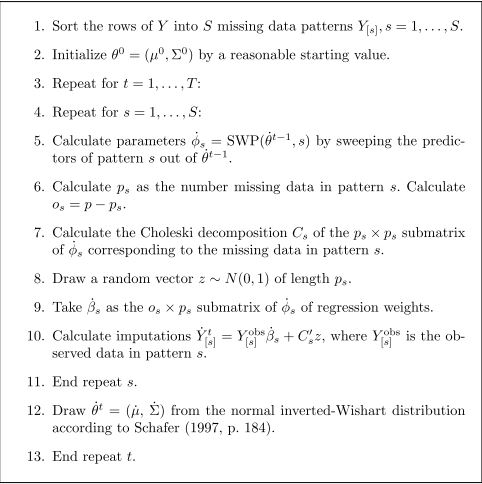
\includegraphics[width=0.8\textwidth]{jm_algo}
  \caption{Normal JM imputation pseudocode}
\label{fig:jmexample}
\medskip
\small
Taken from van Buuren's book �Flexible imputation of missing data� \cite{VanBuuren2012}
\end{figure}

There has been extensive programming and research on using the normal model for JM, and research shows that it even performs well under situations where the data has strong non-normality \cite{Demirtas2008}. Not much research has been done on models outside of the normal. 

This is just one implementation of a JM approach. Another, like that used in the Amelia package, uses an EM algorithm to draw from the missing data's posterior assuming a normal likelihood and user specified priors \cite{Honaker2015}.  Other distributions can be used, but the user will have to specify it, derive any relevant distributions, program it, and research to see if the method provides optimal properties, such as proper coverage and correct estimation of the parameters of interest.

An obvious issue with JM arises when the data is categorical (either alone or mixed in with continuous). There has been much debate in the literature about how to handle this situation. Some authors argue that you should just impute under a continuous distribution and round imputations to the nearest category number, and others suggest using distributions that are more suited for categorical data \cite{VanBuuren2012}. However, no consensus has been reached on the best method. The issue still remains that JM handles mixed data very poorly.

\begin{comment}
A few of the most used R packages for joint modelling imputation include Amelia \cite{Honaker2015}, norm \cite{norm2015} and cat \cite{cat2015}.
\end{comment}
It is my opinion that unless the user is very confident in the multivariate joint distribution of where the data comes from, that JM should not be used. While JM is theoretically sound, its assumptions are so strict that it is nearly unusable in practice. In the cancer example, there are many categorical variables and strictly positive variables to impute, so JM seems inappropriate.

The other MI strategy is called fully conditional specification (FCS). In this paradigm, missing data is assumed to be MAR (although it can work on MNAR with more assumptions), and is imputed on a variable by variable case on the columns/covariates based off of user specified imputation models. Whereas JM imputes on the rows, FCS imputes on the columns. Imputations are drawn from the missing data's posterior predictive distribution. This theory goes by many names, including partially compatible MCMC, iterated univariate imputation, and chained equations \cite{VanBuuren2012}. In the JM setting, the user must give one $p$ dimensional model, however in the FCS setting, the user must give $p$ one dimensional models. The goal of FCS methods are to sample from
%I take out the X's here to keep consistent with the apdx
$$P(Y,R|\theta)$$
By sampling from the full conditionals
$$P(Y_j|Y_{-j},R,\phi_j)$$
In this notation, $Y$ is the fully observed data, $ Y_{-j}$ means all of the columns of the data except for $j$, $R$ is the missing data indicator,$\theta$ is the vector that parameterizes the full data model, $\phi$ parameterizes the imputation model . A pseudocode example can be seen in figure \ref{fig:fcs}.  This method is called Multiple Imputation by Chained Equations (MICE), and draws the imputations from the posterior predictive density of each missing covariate in an iterative fashion. The imputation models in step 1 can either be parametric distributions, or models (such as regression, predictive mean matching, etc.), that are specified by the user. Note that the previous imputations enter the current imputation only through the relation with the other variables (step 5), and not directly. Because of this, convergence is often seen within 5 iterations \cite{VanBuuren2011}. The values at the last iteration are taken as the draws from the missing data's posterior, and these are the values used to fill in the missing data.

\begin{figure}[h!]
  \centering
    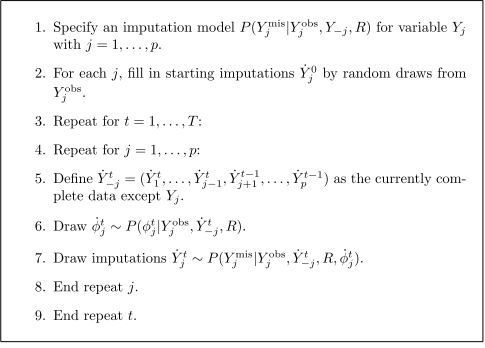
\includegraphics[width=0.8\textwidth]{fcs_algo}
  \caption{MICE FCS imputation pseudocode}
\label{fig:fcs}
\medskip
\small
Taken from van Buuren's book �Flexible imputation of missing data� \cite{VanBuuren2012}
\end{figure}

One of the major criticisms of this method is that in order for there to be a guarantee that we are sampling from the correct distribution, we need to ensure that our full conditionals are compatible, i.e. that they factor into the proper, explicit joint. This is very hard to check in practice, but multiple studies have shown that even when the models are highly incompatible, FCS methods are very robust and produce proper imputations \cite{VanBuuren2006}. FCS allows us much more flexibility than JM does since each model is under the users control, and it handles mixed categorical and continuous data much better than JM does \cite{Kropko2014}. In addition, specifying the individual model for each covariate allows the user to handle the intricacies of each covariate.

\begin{comment} Some popular R implementations of FCS methods include MICE \cite{VanBuuren2011}, mi \cite{Su2011}, and BaBooN \cite{Florian2015}, which go about drawing from the posteriors in different ways. These methods are good, but I will be using MICE in the applied section of this paper.
\end{comment}


The user is going to have to specify something, there is no escaping that, but it is easier for the average person to be able to define a single distribution and model rather than to guess at a multivariate distribution, particularly if it is high dimensional. In addition, in the survival analysis setting, there will naturally be strictly positive and categorical variables. Trying to fit a parametric distribution with these stipulations will be very hard if not impossible, so we will be relegated to using a general distribution (like the normal), which will certainly elicit a poor fit. So, JM approaches certainly seem ill-fitting, however FCS approaches are very appealing. 
\begin{comment}
In an ideal world, we would have complete data, and would not need to resort to imputation. But since we don't have complete data, we must choose one method and accept its strengths and weaknesses.
Might want to move elements of this down to application
Now that we have chosen the paradigm, we need to select an implementation of it. Many exist (such as MICE \cite{VanBuuren2011}, mi \cite{Su2011}, etc.). I wanted to select the implementation that combined ease of use, understanding, and programming. What I decided upon was a method called MICE- Multiple Imputation by chained equations \cite{VanBuuren2011} MICE is an FCS MCMC method that under compatibility, is a Gibbs sampler, where we obtain samples from the joint by sampling from the full conditionals. The user defines the full conditionals, so it is possible that the joint may only exist implicitly, and not actually have a functional form. 
\end{comment}

In order to use FCS methods properly, the missingness in our data must be MCAR or MAR. It can work with MNAR missingness, but it requires some extra modelling assumptions that are beyond the scope of this thesis. T tests have been proposed to test if the data is MAR or MCAR, but this is of little use for us, because we only want to know if the data is MNAR, which is impossible to test since testing for MNAR would entail us using information that is impossible to get \cite{Enders2010}. Luckily, we can safely assume MAR if there is reason to believe that some of the covariates collected account for the missingness \cite{VanBuuren2012}.


It should be noted that in the real data we will use, the response variable (survival time) is fully observed, but the covariates have a lot of missingness. If it were the case that we had missingness in the survival time, then the methods described above might not work. They might fail because the unobserved times or outcomes may follow a different distribution than the observed times. This is cleared up by Zhao et. al in 2014 through Kaplan-Meier MI  \cite{Zhao2014}. This is beyond the scope of this report though so I omit its details. 

\subsection{Setting and Checking the Imputation Model}
Once we have checked that the MAR assumption is true, we need to set up our full conditional imputation models. This may take a while for large datasets, but the extra time spent will ensure a better and move valid imputations. We choose what method to use (regression, predictive mean matching, logistic regression, trees, parametric distribution, etc.), and then what predictors will go into those models. We should choose predictor variables that help explain missingness, as well as those we are doing inference on, as to avoid bias \cite{VanBuuren2012}. For variables that are derived from others, we impute its components and then compute that variable, in a process known as passive imputation. With large datasets, we may need to perform variable selection before specifying the models, so that setting up the models doesn't become unmanageable.

Since FCS is an iterative process, we must choose how many iterations to do until convergence. The older literature suggests 5 iterations are enough, but with modern computation, we can easily exceed this, even with large data \cite{VanBuuren2012}. A good way to assess how many iterations to run is to look at the trace plots of the imputed values and then add 5 iterations to the number at which we assume convergence is achieved. Due to the nature of FCS methods, convergence is often very quick, often as soon as 5 iterations. As well, we need to decide how many datasets to impute. The early literature argued that 5 datasets would suffice, but modern literature argues for more, since it will cut down on simulation error. With the speed of computers and availability of storage, many authors now suggest using more than 5 imputations \cite{VanBuuren2012}. Many different authors have different criteria, but a popular criterion is to impute as many datasets as the 100 times the percentage of cases in the analysis with missingness \cite{White2011a}. 

Once we have determined how many iterations and imputations to run, the FCS algorithm is ran. Depending on the model specifications, it should not take too long for small datasets (seconds or minutes), but may take hours for larger ones. FCS models often converge quickly, so after convergence, we are just taking draws from the missing covariates posterior. The first few iterations may be considered as burn in, and the rest as samples. The value at the last iteration of each chain is taken as the sample from the posterior that will be used as the value for the missing data.

We need to verify that our imputations are valid once we complete them. First, we need to see if our chains have converged. Since FCS methods are  MCMC method, we should check the chains for irreducibility, aperiodicity, and recurrence. To determine when the chains have converged, van Buuren suggests that ``Convergence is diagnosed when the variance between different sequences is no larger than the variance within each individual sequence'' \cite{VanBuuren2012}.  There is some research (but not from the MI perspective) about tests to check for convergence, and a popular test is Gelman and Rubin's $\hat{R}$ scale reduction factor test \cite{Gelman1992}. This test is often used in conjunction with visual tests.  Assessing convergence  by looking at of all of the values over $m$ imputations and $k$ iterations would be very hard to visualize because there would be so many chains, so often times, we will choose to observe a statistic (like the mean) of the chain and assess on that. 

Once convergence is assessed, we need to check that the values imputed are valid and come from the correct posterior. This will serve as our model checking and validation. The overarching idea that we need to pay attention to is �does the data look like it could have been real data�. We can assess this in many ways, including density plots, box and whisker plots, scatterplots, histograms, etc. This is a visual task and there is no statistical method to validate this.

This whole process can be very time consuming because every time we want to make a change in the methods used, we have to rerun the algorithm and reassess our results. But once we find the setup that works for us, we don't need to repeat it again. So, while it may take a lot of time now, setting up a proper model will save us even more time in the future and ensure that our imputations are valid.

\subsection{Combining the MI Estimates}
Once the $m$ datasets are imputed, we may run any valid analysis on each imputed dataset \textit{individually}, treating each of the $m$ datasets as if it was complete. Of course, the analysis in question should be run on the available cases, to ensure that the model assumptions are reasonable. We will speak about what exact analyses will be run in the next sections, but for this section, we focus on how to combine \textit{any} analysis.

\begin{comment}
I am a strong advocate of running the model with the available cases if possible before running it on the MI data, so that we can assess the appropriateness of the model. As well, running the model with the available cases will give us a clue as to what to expect from the MI analyses (such as sign of the coefficients or level of significance).
\end{comment}


The idea of what we would like to do is to take the $m$ estimates of the scientific estimand in question, and pool them down into one single estimate. Rubin's rules are a set of rules that guide us in making inference from multiply imputed data. They will give us a single point estimate for the scientific estimand in mind, as well as the proper variance for it from the $m$ imputed datasets \cite{Rubin1987}.  
%Do I need to make this bold?

Rubin's rules involve three parts. The first is getting an estimate of the population estimand $Q$, estimated with the MI datasets by $\bar{Q}$. To get $\bar{Q}$, define $\hat{Q}_i$ as the estimand evaluated from the data in the $i^{th}$ dataset.  Then, take the average over all $m$ datasets to get a single estimate $\bar{Q}$.
$$\bar{Q}=\frac{1}{m}\sum_{i=1}^{m}\hat{Q}_i$$
The estimates are not set, and there is variance associated with them. The first form of variance is the ``within'' variance, or the variance of each estimate $\hat{Q}_i$. This is the typical variance observed from having a sample. Define the variance covariance matrix of the $i^{th}$ imputed dataset as $\mathbf{\bar{U}_i}$ , then the estimate of the within variance is computed as
$$\mathbf{\bar{U}}=\frac{1}{m}\sum_{i=1}^{m}\mathbf{\bar{U}_i}$$


The last form of the variance is the ``between datasets'' variance. This is the variance associated with the fact that we have missing data. It is given by
 $$\mathbf{B}=\frac{1}{m-1}\sum_{i=1}^{m}(\hat{Q}_i - \bar{Q})(\hat{Q}_i - \bar{Q})'$$

The total variance for $\bar{Q}$ is given by 
$$\mathbf{T=\bar{U}+B +\frac{B}{m}}$$
The last term is our simulation variance, and its existence is proven by Rubin in \cite{Rubin1987}.

The theory of inference with Rubin's rules is rooted in the assumption that under repeated sampling, the complete data quantity of interest is $Q-\hat{Q}$ asymptotically normally distributed with mean 0 and variance $U$, where $U$ is the variance of $(Q-\hat{Q})$ \cite{VanBuuren2012}. We don't have the true population variance, so we must use what we have from the sample, namely $T$, the MI total variance. With this assumption, we know that
$$\frac{Q-\bar{Q}}{\sqrt{T}}\sim t_{\nu}$$ 
And the degrees of freedom is proven to be 
$$\nu=\frac{\nu_{old}\nu_{obs}}{\nu_{old}+\nu_{obs}}$$
Where $\nu_{obs}=\frac{\nu_{com}+1}{\nu_{com}+3}\nu_{com}(1-\frac{B + B/m}{T})$
, $\nu_{com}$ is the hypothetical complete sample degrees of freedom, and $\nu_{old}=\frac{m-1}{(\frac{B + B/m}{T})^2}$ \cite{Barnard1999}.

Rubin's rules assume normality, so if our statistic in mind is not asymptotically normally distributed, then we need to transform it towards normality before pooling. There have been some research about how to pool non-normal quantities, but current research shows poor results and power when doing so \cite{Marshall2009}. Using Rubin�s rules, we now have a powerful framework to get a single, valid estimate from multiply imputed data.

It should be noted that while Rubin's rules are the most popular method to combine MI estimates, there is another way to work with the multiply imputed data. This method is colloquially called the �stacked method�. For the stacked method, we take all of our imputed data and �stack� them one on top of each other to get one huge dataset of size $(m*i)$ rows and j columns. Under the stacked method, unbiased estimates of quantities of interest can be produced, but the estimates of variance will be too small (since we are artificially increasing the sample size) \cite{VanBuuren2012}. Thus, the stacked method is a poor choice for running any hypothesis tests or quantifying uncertainty. It is not useless though. The stacked method is useful when we want to analyze just one plot instead of $m$ for model checking. As well, the stacked method may be useful in situations where we partition categorical data on an imputed variable and then look at the percentage in each category. Under the averaging portion of Rubin's rules, we are not guaranteed that the percentages will sum to unity, but under the stacked method we are.


\section{Survival analysis}
\label{sec:Surv}
Now that we have the multiple imputation datasets created, we may run our analysis on each of them. Since the goal of this paper is to analyze cancer survival data, it naturally follows that the models we would like to run are survival models. As a general rule of thumb, we should run our desired analyses on the original available case data to get the available case estimates, as well as to get an idea of what to expect and to check if the model assumptions are met. Following Rubin's rules, we run the individual analyses on each of the $m$ datasets, and then pool our results. In this section we will discuss each type of survival analysis and how to use them in the MI setting, as well as the issues associated with them.

\subsection{Kaplan-Meier Survival Curve}
Analysis for the Kaplan-Meier estimate is quite simple in the non-MI setting, but special care should be taken in the MI setting. First, we need to clearly define what the groups and population are, and what constitutes an event of interest. A very common mistake that researchers make is to try to frame a competing risks problem as a Kaplan-Meier problem. We also need to be sure that we have non-informative censoring, that is, knowing that the individual is censored tells us nothing about their survival probability. Once we have checked all of these, we can compute the Kaplan-Meier curve on each of the $m$ datasets. For simplicity, in this section we assume that the Kaplan-Meier curves are run on a dataset with only subjects who took either a treatment or a control. Now, we could pool these estimates, but that would be ill-advised because the Kaplan-Meier curve is not normally distributed. To get around this, it has been proposed by Marshall et. al to take the complimentary log-log transformation of the Kaplan-Meier estimates before pooling \cite{Marshall2009}. We can make this transformation, pool our results, and then back transform to get the pooled MI Kaplan-Meier estimate. 

In the MI setting, an interesting situation may arise when the last event (and thus the range of survival time) differs between the imputed datasets. This is the result of a person with a long survival time being put in different groups via imputation. We can deal with this by either extending the last observed Kaplan-Meier estimate out until the last event time,  truncating all of the imputed curves at the minimum time of last event, or using other methods to deal with this situation as described in reference \cite{Klein1984}. In traditional analysis, we would not extend out the Kaplan-Meier curve out past the last event, but if we have wildly varying imputations, this might be a good option, so that we can make inference between curves and are not hampered by one poor imputed dataset. As well, we could use the stacked method to get the Kaplan-Meier estimates, but we must accept the fact that the variance at every time point will be too small.  The decision of what to do is up to the researcher and depends on the nature of the problem. 
\subsection{Median Survival Time}
Once the Kaplan-Meier curve has been estimated, one of the main tasks that clinicians are interested in is the median survival time of each group, which is the smallest time that the survival function for the group is less than 0.5. Since the true survival function is unknown, the Kaplan-Meier estimate is used. The median is the preferred method of central tendency in survival analysis because often times the survival times are right skewed, making the mean a poor estimator of the truth. Finding the median in the MI case is quite simple, as it is the first time that the pooled MI Kaplan-Meier curve crosses below 0.5. We would also like to have the variance at the median. The first way to obtain it is to multiply impute the variance (i.e. make the variance the scientific estimand of interest), and then use Rubin's rules to get the variance associated with each time point and then take the average as the variance at that time point. However, taking the mean and variance of the variance doesn't make much sense, and under typical pooling of the Kaplan-Meier estimate, we already get a good estimate of the variance. A better solution for this issue is to derive the variance of the median by the ``reflection method''. In this method, we first fit the MI Kaplan Meier curve, and then construct a 95\% confidence interval for all time points using the total variance obtained from Rubin's rules pooling. The median is defined as the first time when the pooled MI curve crosses 0.5, and the lower and upper 95\% confidence interval for the median are the medians of the upper and lower confidence bands. This method is preferred because it uses the variance we actually have and is much more robust to poor imputations.


\subsection{Log Rank Test}
Now we have a pooled estimate of the true survival curve for each group. In the typical setting, we might want to look to see if these curves are similar to each other, so we can determine if the treatment really prolongs survival time. We would do this with the log rank test under the regular setting. However, we should not be deceived. We have an MI pooled survival curve, which is not constructed in the same way that a regular Kaplan-Meier curve is. Because of this, we cannot get the quantities that we would need to compute the log rank test. However, we can still get the MI pooled log rank test. To do so, we can do one of two things. The first is to run the log rank test on each of the MI datasets and then pool the results via Rubin's rules. This is the logical way to do it, but under this scheme we will run into a multiple comparison problem. As well, Marshall shows that this method is unreliable and will not give the proper p-values \cite{Marshall2009}. Another option is to run a Cox regression on just the treatment indicator and then compute the score test statistic, since this is equivalent to the log rank test under no tied failure times \cite{Klein1984}. Under tied failure times, they are very similar to each other. From the Cox regression, we can obtain the score test for each of the datasets. We could pool the score test from each MI dataset, but we will once again run into problems with the actual pooling. We could also try to run the score test on the pooled MI Cox regression model, however, in order to do this, we need to know who is in the risk set. But the concept of a risk set doesn't exist in the MI setting. Luckily, the Wald test is asymptotically equivalent to the score test, and the Wald test is very easy to obtain.  So we can use the Wald test of the coefficient from the Cox model as a proxy for the log rank test. In this way, we get a statistic that calculates what we want, while still making sense in the MI context.
\subsection{Cox Proportional Hazards Model}
We would now like to investigate the hazard ratio of different baseline covariates and treatments via the Cox proportional hazards model. The overall goal will be to fit a Cox model with baseline covariates, check to see if it passes the proportional hazards assumption, and then add in the treatment variables to see how they affect the hazard. It is known that the Cox regression coefficients are normally distributed, so there is no issue in pooling, but we do need to be careful about checking the proportional hazards assumption. The very first thing that we need to do is check to check the available case model to assess if we have proportional hazards. If one of the covariates truly is dependent on time, adding imputed data isn't going to change that, so checking the available case analysis is a good sanity check. The way we go about checking to make sure that we have proportional hazards is looking to see if the Schoenfeld residuals are uncorrelated with time for each covariate in the Cox model \cite{Schoenfeld1982}. The Schoenfeld residuals are tedious to explain and derive, and add no value to this thesis; however knowing that they are partial residuals that that are formulated to be independent of time should suffice to understand this paper.  The most common way to determine proportional hazards is to plot the spline fit (often cubic) to the residuals along with the 95\% confidence intervals, and see if any straight line could pass through the bounds. Because the residuals are independent of time, a straight line over time signifies that the hazards are proportional \cite{Schoenfeld1982}. There isn't an official name for this method, but the straight edge method seems to be a fitting name since you can check it by placing a straight edge between the confidence bands. If this is the case, then we say that that the covariate in question does not depend on tine, and follows the proportional hazards assumption. Another method to check for proportional hazards is to use a chi square test of independence between the Schoenfeld residuals and time, although this is rarely used in practice.

If the proportional hazards assumption is not met, then we can add the variable that does not have proportional hazards into the model as a time dependent covariate. This is beyond the scope of this thesis, but is something that could certainly appear in practice.

We have discussed how to check the proportional hazards assumption in the available case scheme, but how can we do this in the MI setting? We can take our imputed data and fit a Cox model on each of the $m$ datasets, and pool them easily. But how is the best way to check the proportional hazards assumption? We can go about this in a few different ways. The first is to check the proportional hazards assumptions on each individual MI dataset. This may prove to be an arduous task especially with large $m$ and a large number of covariates in the model. Alternatively, we could superimpose all of the spline fits on one plot, and see how the shape and general trend compare to the available case analysis. We can also use the stack data to get just one set of plots, but the straight edge method will not work here since the errors are too low. 

Once we have verified that the model follows the proportional hazard assumption, we may trust its results. We can now add in our treatment covariates, and analyze it to see how they affect the hazards.

\section{Causal Analysis}
\label{sec:Propscore}
Now that we have laid down the theory for analyzing the survival section for clinical relevance, we can move on to the causal analysis part. Viewing the analyses with a causal lens is important, because as of now with only survival analysis, we cannot be sure if the differences in treatments are actually due to the treatment or to some differences in the groups before they even received the treatment. While there is a lot of preparatory work that goes into the theory of it, the results that can be obtained using causal analysis framework and propensity scores is much stronger and appealing than conventional analysis.  Although no statistical method will give us a causal relation, the results from causal analysis will be much more similar to the results we would have got from a RCT.

Propensity score methods are an easy to understand yet powerful tool to help implement Rubin's causal model. The use of propensity scores justified in Rosenbaum and Rubin's 1983 paper \cite{Rosenbaum1983}.  Our overall goal is to estimate the average treatment effect in a setting where the initial study was not an RCT. We will use the propensity scores to balance the groups and remove the effect of confounders, so that the data seems more like an RCT. 

Before we even begin using propensity scores, we should have in mind what estimand we wish to estimate (the ATE or the ATT). It should be noted that while the ATE and ATT deal with means, the definition can be modified so that it can deal with the difference in hazard ratios \cite{Austin2014}. The choice of estimands should be done by addressing the problem and discussing the implications of each with subject matter experts. Once we have this, we can start out with the propensity score methods. 

\subsection{Selecting the Method}
We will need to make many decisions along the way, both in how to use the propensity scores, and how to combine them with the MI data. There are four main uses of propensity score in the literature: matching, stratification, weighting, and covariate adjustment \cite{Austin2014}. The goal is to balance the treatment and control groups, such that the only difference between the groups is due to the treatment received, and not any underlying factor. All of these methods will help us to examine the average treatment effect, but each goes about it in a different way. Covariate adjustment and matching have fallen out of favor in the literature recently, but weighting and stratification remain very popular \cite{ Austin2014}. We will be using weighting in our real data analysis, so the main focus will be on that, but the methods discussed will work with any propensity score method. Whatever method is chosen will need to be run on the MI datasets. 

Since the stacking method will not work for propensity score analysis (there will be a falsely inflated sample size), we must decide how to use propensity scores on the multiply imputed data. Two methods are described in Mitra and Reiter about how use propensity scores in the MI setting \cite{Mitra2012}. In both methods, the propensity scores are first computed for each MI dataset, as we would normally do in the analysis part of the MI process. However, how the two methods use the propensity scores are different. In the first method, known as the ``within'' method, the propensity score method is done within each MI dataset and then pooled. For example, if we wanted to find the ATE, we would estimate the ATE in each dataset, and then pool via Rubin's rules. The other method, known as the ``across'' method, takes the $m$ estimates of each individuals propensity scores between the MI datasets, and then averages them so that every subject has one averaged propensity score. Once the global averaged propensity scores are estimated, then the propensity score method is used in each dataset (using the global list), the ATE is estimated on each dataset, and then pooled via Rubin's rules. Both methods have their pros and cons, and are appropriate for different scenarios. 

\begin{comment}
However, the treatment variable may itself have missingness, and thus needs to be imputed. In this situation averaging across datasets does not make sense (since there is no guarantee that a given subject in imputation $i$ has the same treatment in imputation $j$), so we cannot determine if the subject is a case of a control, thus matching will be impossible. When this is the case, we must use the within method. 

\end{comment}
%does the fact that the drug is an imputed value effect which model we should use? The problem exists %that the treatment is unknown in some, so it needs to be imputed.  Thus, we could have 30 datasets %where subject I is treatment, and 20 where he is a control. We can either classify as treatment via %majority voting. If not this, then we need to change to the within method.
\subsection{Obtaining the Propensity Score}
Now that we have discussed how to use propensity score methods in the MI setting, let's discuss how to actually get the propensity scores for each MI dataset. From now on, propensity score weighting will be the only method discussed, because that is what will be used in the application section. However, the framework will still work for other types of propensity score methods.

Different propensity scores will be obtained according to what pretreatment covariates we use in the propensity score model, so we need to be sure that model is fit with clinically relevant and meaningful predictors. Recall that our overarching goal is to account for any pretreatment covariate that confounds the selection of the treatment, and to try to make the no unmeasured confounders assumption more reasonable. Basically, we would like to control for everything that could be different between the two groups. There has been significant debate among statisticians about how to set up these models, by either throwing in every possible variable into it, or only include covariates known to affect treatment selection. I don't plan to settle this debate, but I do believe that the user should account for everything that is believed to be different between the two groups in question, in order to make the no unmeasured confounders assumption more plausible. 

Obtaining the propensity scoring using logistic regression is simple and has been historically used, but with newer machine learning methods, we are able to get better propensity score weights that induce more balance (which will be talked about next). For single analysis, logistic regression would be preferred due to its simplicity and power, but in the MI setting, the model that fits well for one dataset might not fit well for another one. That is why machine learning methods are preferred. In recent years, boosting has become very popular method to compute propensity scores, because they can be selected in a way to achieve optimal balance between the groups, while also remaining simple and theoretically sound\cite{McCaffrey2013}.

\subsection{Verifying Balance}

The goal of weighting is to create a pseudo-sample that is balanced, by up weighting samples that look like treatment cases, and down weighting those who do not. The formula for each weight can be concisely given as $w_i=\frac{T_i}{\hat{e}_i(x)}+\frac{1-T_i}{(1-\hat{e}_i(x))}$, recalling that $T_i$ is the treatment indicator, so only one of these terms is ever not 0. Two methods have been suggested to check for balance. The first is known as standardized bias. For each pretreatment covariate we wish to balance, we see how similar the cases and controls are by observing $|\bar{X}_{k1}-\bar{X}_{k0}|/ \hat{\sigma}_k$, where the barred X's denote the propensity score weighted means of the covariate in the treatment and control groups, and the $\hat{\sigma}$ is the unweighted standard deviation of both groups together. Typically, standardized bias below .2 or .25 indicates good balance, although this number is subjective. Another common method is the Kolmogorov�Smirnov (KS) test of distributional equality. In this nonparametric test, the Empirical Cumulative Distribution Function (ECDF) is computed for the two (weighted) groups. Then, the maximum distance between the two ECDF's is calculated. Its p-value is found via the permutation test for the null hypothesis of no differences in the distribution \cite{McCaffrey2013}.


Both of these methods offer us tools to assess balance in the data when weighted by the propensity scores. We can use the tools to our advantage alongside of a boosting algorithm to get good balance. In boosting, a simple piecewise linear function is fit to the data, and after every iteration, a new piecewise linear function is fit to the previous models residuals. We can boost our data, weight each observation by its propensity score, and then check the balance at each iteration of the boosting algorithm. The goal is to find the propensity score weights that minimize either the standardized bias or the KS statistic, although minimization of one often leads to significantly better balance in the other metric.

Once we have obtained our optimal propensity scores for each MI dataset, we weight the data by them. Then, we check to see if we have balance. As well as checking that we truly have achieved balance, we also need to look at the distribution of the propensity scores. We would like to see some overlap between the treatment and control propensity scores. Overlap indicates that subjects in both groups are similar to each other, and can be compared. If the propensity scores don't have any common support, then we have not properly balanced. We should also be sure that all of the propensity scores are bound between zero and one. If a subject has a propensity score that is either one or zero, then they will always be or never be treated, and estimating the counterfactual will be impossible.

Once we have our propensity scores, we need to go about checking the treatment effect. We have no guarantee that the model we set for our propensity score is correct, so many authors advocate including the covariates in the propensity score model in the analysis of the treatment effect (this is known as a doubly robust method) \cite{Lunceford2004}. 

Now that the theory is set up, we may use it on the MI data. And now we may interpret the results with a causal lens, even though the data may be observational. We will be using the ``within'' method, so for each MI dataset, we compute the treatment effect from the propensity score weighted data. While we could check the treatment effect in terms of time difference in survival between the treatments, this doesn't work very well, because we have censored data. The better option is to observe the average treatment effect by looking at the change in the hazard between the treatment groups. Checking the hazard makes use of the fact that we have censoring in the data \cite{Austin2013}. We may then combine the estimates via Rubin's rules to get the MI estimate of the average treatment effect and its variance.
\begin{comment}
The matching can be done in many different ways like a nearest neighbor, caliper, or mahalanobis distance matching. It shouldn't really matter which one we use, so long as the groups are similar in distribution after matching in each dataset.
Once an acceptable propensity score model is selected, we will need to pick what type of weighting we will do. Many exist, but the most popular are X,Y,Z . We will then run our Cox model again (as in the survival section), but we will factor in the weights. Then, the results that we receive can be viewed as if they were from a RCT. As well, we can go ahead and analyze them as such, and draw causal inference. I need a lot more work here.

\end{comment}


\chapter{Application}
\section{Data Explanation}
\label{sec:data}
\begin{comment}
We have now laid down the theory of what we want to do describing all of the choices we may need to make, so now we will put it in action. The data that we will apply it to is a dataset from M.D Anderson Cancer Center. The data is a collection of about 1500 patients at MD Anderson who have breast cancer that has metastasized to the brain, about 100 clinically relevant covariates, along with their survival status and time.
\end{comment}
Unfortunately, as of October 16th, we are still waiting for final approval from the PI of the project and the IRB. I want to get the proposal out to y�all though. So, what I will do in this section is describe what I will do, and once I get approval, I will fill in the tables and plots. In the meantime, I will put in <whatever> where something that uses the data should be. The IRB protocol is RCR03-0931, but neither Dr. Hess nor myself are on the protocol, because it is out of date. We are in the process of getting it updated.

Now that we have the theory in place, we can apply it to some real data. The dataset that I chose to analyze is a dataset from MD Anderson Cancer Center, with permission from Dr. Bugano, Dr. Ibrahim, Dr. Hess and <whoever else needs to be thanked>. This dataset has historical records of 1514 MD Anderson patients who have had breast cancer that has metastasized to the brain. There are lots of covariates recorded (about 90, with some missingness), a few different treatments, as well as survival endpoints (which are all observed). This data is exemplary for this task because it is large, survival amenable, has missingness and is a prime candidate for imputation, and has treatment variables that are not given in an RCT. <plot and table  of missingness> 

Our first step is to clearly define what we would like to find. There are many interesting questions we could ask and answer from this data because of the amount of data available, but the question I will focus on here is the effect on survival and treatment of two HER2 (breast cancer grown protein) therapeutic drugs-Lapatinib and Trastuzumab (or do I want to do capecitabine/other/none). It isn�t vital to understand what these drugs do, but the interested reader may want to look at  appendix \ref{app:apdxb} for a very basic overview of cancer and the methods of how these drugs work. For a much more detailed analysis and other clinically relevant questions, see !!Hess, Bugano, Berliner!! This is the project that this research was forked off of, although it will probably not be published by the time this thesis is. 
\section{Imputation}
%start here
We first need to impute the missing data. This is a challenging task, because of the attention and care that needs to be given to imputing about 90 covariates with missing data. But we need these covariates to be imputed properly because; they have the potential to be useful as predictors for other covariates, they might be something we are actually analyzing (now or later), we have spent the money to collect the data, and it strengthens the MAR assumption. As well, it is my opinion (and probably a consensus among applied statisticians) that is better to have too many covariates than not enough. After all, we can always use variable selection if we have too much data. 

Our data is quite high dimensional, and there are a many binary variables, thus JM imputation seems inappropriate. Instead, FCS models seem better suited. We will be using the R package mice \cite{VanBuuren2011} because it is easy to use yet powerful. 

The model is set up by hand, following the advice from \cite{VanBuuren2011}. It took a about three weeks to set up and check. This was because the number of covariates was huge, and checking the imputations after a change was time consuming. It would not take this long for a smaller dataset. Creating valid imputations is a skill that lies somewhere between an art and a scientist, so it takes the theory to know what to do, and trial and error to see if you�ve done it correctly.
%start here
For each covariate with missingness, we need to decide what method will be used for imputation, and what predictors will be used in it. I decided to be very forgiving, and use nearly every predictor for each missing covariate. I did this to bolster the MAR claim, and avoid variable selection. As well, the appropriate methods need to be selected for each datatype. The majority of the data is categorical, so decisions need to be made about whether to impute them via predictive mean matching or logistic regression. This decision was made by observing density plots after the algorithm was run to see if the imputations for each kind were valid. As well, derived variables were coded in as passive imputation, so that they would not be imputed, rather they would be computed.

After the model has been set up, we need to run it and save the results. For 50 datasets, 40 iterations, the algorithm runs in about X hours, and for 50 datasets with 100 iterations, it took Y hours on a computer with Z ram and Q processors. While this seems like a long time, this process only needs to be done once and requires no human interaction, so it can be run overnight and then never need to be touched again. For the rest of the analysis, I choose to use the 50 datasets, because there is hardly any confidence going from 50 to 100, and having such large objects in memory can be harder to work with.

Once the mice algorithm has run, we need to check for convergence and reliability. Convergence is assessed by looking at <plots of covariate mean and sd by iteration>. According to van Buuren �the different streams should be freely intermingled with each other, without showing any definite trends. Convergence is diagnosed when the variance between different sequences is no larger than the variance with each individual sequence� \cite{VanBuuren2011}. Looking at these plots, this certainly seems to be the case. Other authors suggest using a more formal statistical tests such as <rhat> to assess convergence, so I also display that (values near 1.00 mean ok and values greater than 1.1 indicate we should run longer). Diagnostic plots are viewed to ensure that the imputed data is similar enough to the real data.< A few of the plots have been replicated here>. To see all of the plots, go to the shiny app/ R package (do this if enough time, also see about security. Might just need to make it be �available upon request�). As we can see, not all of the imputed data follows the distribution of the observed data exactly, but we obviously don�t expect this to happen always. For the majority of the plots though, the data look like they could have been real data.
\section{Survival Analysis}

Now that the datasets are imputed, we are ready to run our models on them.  As a sanity check, we may compare the fitted models to the available case analysis. Since the imputed values we generate ought to be quite similar to what data we have (unless there is reason to believe that the missing data is significantly different than the observed data), we should expect our estimates to be similar.

It should be noted that in all of our survival analyses, we will be doing a landmark analysis. Landmark analysis means that we don�t start the analysis at time 0, rather, we start it at a different time. In Dr. Hess�s words, �Since the brain met treatment data was necessarily determined after the diagnosis of the brain met, it is not appropriate to use this data as baseline covariates in the analyses. Only covariates known at the time of diagnosis can be used in this fashion� we can do a landmark analysis by estimating when the vast majority of patients would had their brain met treatment choices started and starting our analyses at this point�. After speaking with subject matter experts (Dr. Bugano and Dr. Ibrahim), this landmark time was determined to be 2 months. 

The first result that we will check is the Kaplan Meier curves for the imputed data. The available case analysis shows that lapatinib and trastuzumab are quite close to each other, while having no her2 directed treatment being much lower. The logrank test statistic is X. The pooled KM estimate was found using Rubin�s rules, but under a complimentary log-log transform as suggested by \cite{Marshall2009} to get the survival curves towards normality. The results from MI look quite similar <AC analysis and MI analysis>. We can also get an approximation for the log-rank test on the MI data via the Wald test on the pooled Cox model (NOT the Kaplan-Meier model, Kaplan Meier is not normally distributed, and no obvious transformation exists to make it so, so we must use Cox). We are not able to get the exact log-rank test because in doing so, we would need to compute either the likelihood ratio test or score test, both of which would include calculating the risk set, which is not possible in the MI case. Another suggestion is to pool the chi square statistics via methods presented in Marshall et al 2009, but even they say that this method is poor \cite{Marshall2009}. So, our only real option is to use the wald test (which is very easy to compute), and use that value as a proxy for the log rank test (they are asymptotically equivalent).

!!!Do I want to do competing risks analysis? I will if I have time!!!

Now that we have estimate of survival, we may set up a model to observe how changes in some baseline covariates change the hazard. We will do this with the Cox Proportional Hazards model. Once we have a baseline model fit and the assumptions met, we can add our treatment variable to see how this affects the hazard. The original available case model is as follows.  We need to make sure that the proportional hazards assumption is met, so we may check the cox zph command to look at the schoenfeld residuals over time, and check the test stat. Overall, the assumption of proportional hazards over time seems reasonable, and the test statistic affirms this <AC cox.zph plots>. Although the splines fit the points may not look straight, it certainly seems reasonable that a straight line could be fit (denoting a hazard that is constant over time) between the 95% confidence bands (this procedure doesn�t have a name, but it is known colloquially as the straight edge test).  

Now that we have verified that the available case analysis seems reasonable, we can work with the MI data. We fit that same cox model on all of our imputed data sets, and pool our results via Rubin�s rules (no transformation needs to be done since the Cox model coefficients are assumed to be asymptoticaly normal). We need to verify that we still have proportional hazards though. This is not an easy task, since we don�t actually have a model, rather, we have the average of multiple models. We are no longer estimating the parameters by maximizing the partial likelihood; rather we are estimating them based on the average of the coefficients from the MI datasets. There are two ways we can go about this. The first is to check the proportional hazards assumptions on the stacked dataset.  This will give us a good visualization about the shape of the splines fit to the residuals over time, but when running the chi square test to check for the correlation between the coefficient and time, the sample will be artificially too big, and thus we cannot trust the results. The correct way to do this is to observe each plot and statistic generated from the m datasets to see if the assumptions hold. This may seem like an arduous task when the number of imputed datasets is large, but we can circumvent it by writing a shiny app to view them, or <plot all of the splines on one plot>. We can also look at all of the chi square tests for the 50 datasets and 13 variables for each, although there is bound to be some overlap between significance and non significance due to the multiple testing problem. Overall though, our imputed plots are very similar to the plots produced by complete case analysis, to which we have deemed to be acceptable for the proportional hazards assumption. We may now look at the cox regression coefficients and exponentiate them in order to obtain the hazard ratios. Looking at !! table whatever!! , we can see that some factors force a larger hazard ratio than others. We can take the reciprocal of it to look at the protective effects of each covariate. We may then add in our treatment variable to see how it effects the hazard, and see how it changes other factors.
\section{Causal analysis}

Lastly, we will want to draw causal inference, and see what the average treatment effect of each drug is. This is necessary because the data was collected from a database, and we did not have a completely randomized experiment.  As well, this piece of information is what clinicians and laypeople really want�it answers the question of which drug is better. There are many interesting questions that we may ask with this dataset, but here we will only focus on lapatinib vs trastuzumab vs no treatment. The interested reader may read !!my paper!! Upon its publication. The idea for this part of the analysis is to use propensity scores to match subjects and then compare them. As we saw earlier the best way to match is using the X method. There are several R packages to do propensity score matching in R, including X Y Z . I chose to use the X package because of its ease of use. Do a lot more work on this part!!!!!

\chapter{Discussion}
Even though the analyses and interpretations in the survival and causal sections go about answering the question in different ways, the interpretations of them should be clear. For chemotherapeutic treatments, that Capecitabine is not any better than any other chemotherapeutic treatment, but any treatment is better than none. As well, for HER2 directed therapies, it seems that there is no difference between Lapatinib and Trastuzumab, but that both are better than no HER2 directed therapy.

In the analysis, we often talk about ``other'' chemotherapeutic. However, this is not descriptive. In a future analysis, it would be wise to classify the other chemotherapeutic agents, so that analysis could be run to determine which drug is actually the best (in terms of hazard reduction or survival function change). Currently, all we know is that Capecitabine might not be the best chemotherapeutic drug, but we cannot say which is better. 

We have discussed a number of tools and methods to analyze survival data with missingness and make causal inference.  There are lots of decisions to be made along the way, and I am in no way advocating that my exact choices will be proper for all situations, I am only claiming that the decisions made were proper for the type of data and questions that we had. I hope that I have given the reader enough information to run their own analysis, even if they don�t choose the options that I did.

There will certainly be many disagreements about the multiple imputation portion. And since the multiple imputation serves as the root of the analysis, the concerns should be addressed. The first concern comes from people who don�t understand or believe in imputation of missing values. Multiple imputation is a tool to help us find plausible values for missing data. We will make no claim that the imputed values are right, but when used correctly, the results from subsequent analyses will be unbiased. We aren�t using multiple imputation to create data where there is none, rather we are using it to ``fill gaps'' in places that we already do have data. We actually need to impute in certain cases if we want to get valid results, as analysis without imputation will lead to severely biased results \cite{VanBuuren2012}.
\begin{comment}
Might want to put this earlier on
 For example, if teenage males who are obese don�t want to self-report their weight, then classic available case analysis will yield biased results because we have knowingly left out part of the population who are systematically different We need to impute to make sure we have included all of the information and not to bias our estimate.
\end{comment}
The next and more substantial critique will come from statisticians who may not believe that the distribution that the imputations are being drawn from is valid. No matter what method we use to impute, we have to make a parametric assumption, be it the joint model for JM or the full conditionals for FCS.  For our case, using the normal model is certainly wrong because we have so many categorical and strictly positive variables (which is proven to be suboptimal in \cite{Kropko2014}), so we are left only with using FCS. And FCS alone has weak theoretical justification. But as we have discussed before, many studies have shown that FCS is robust to non-compatibility. As well, there was no formal model validation (such as cross validation), only ad hoc checks. In the literature there is hardly any mention of validation, because if we were to cross validate, we would be drawing from different models, and comparison between the folds would be like comparing apples to oranges. We already have missing data, there is no reason to destabilize it to try to compare it, as the standard methods seem to work fine \cite{VanBuuren2012}.

\begin{comment}
An interesting future extension to this project would be to use a non parametric approach to multiple imputation, such as the one suggested by Long et al in \cite{Long2012}. But at the time of publication, there is not much literature or software on this subject, so I felt that it was not appropriate to use its results.  
\end{comment}
To summarize about multiple imputation, I would say that it is a necessary evil. In the process of using multiple imputation, we lose predictive power, and are forced to use a distribution that may not fit the data to a t. But we need to use imputation techniques if we wish to make any sense of our data. The advice I would give to those who are hesitant to use multiple imputation would be to not have missing data, but this is a task that is easier said than done. Multiple imputation is becoming the standard for missing data techniques, especially in the medical field. There are lots of pros to it, but there are certainly some cons. Much research has already gone in to it, but much more needs to be done. It is my hope that this thesis has shown a powerful example of why multiple imputation should be used.

Next we can critique the survival section. We made a lot of assumptions about how our subjects were censored. We assumed that all of our subjects who were censored were right censored and non-informative. This seems to be a valid assumption, but there certainly exists left truncation. It may have been the case that there were some left truncated subjects, but once we landmarked, we certainly incurred some left truncation. When the log rank tests were performed, we needed to use many proxies to actually get the test result. Although it is theoretically justified, intuitively, it is not easy to follow. A topic for future research would be how to optimally combine MI test statistics, because currently the literature on it is slim and the methods are poor.

We decided to use Kaplan-Meier and Cox analyses because they are very standard in practice, and answer the questions well. However, some other methods could have been used. A popular theoretical model is called the accelerated failure time model (AFT), which describes how covariates affect the survival time, assuming that it acts in a multiplicative fashion. As well, we only focused on death data, and did not take into consideration competing risks. Had the dataset been more robust, perhaps we could have incorporated competing risks.  
\begin{comment}
Next, since there is no well-established method to validate the model, we had to be creative and define our own methods to check them. The methods are reasonable and both the stacked and individual methods are very similar. More research should be done though to verify if this will always be the case, specifically in the presence of pathological data. 
We had some survival data in the dataset that would be appropriate for the competing risks setting, but this was not of primary concern to the clinicians. In future research, analyzing this data would be of interest since it poses many interesting problems.
\end{comment}

There are three concepts in survival analysis that I find interesting, but our data did not allow for it. The first is variable selection. The clinicians knew what they wanted to test, so this was not needed, but variable selection in the context of MI is an interesting question, and van Buuren covers it in his book \cite{VanBuuren2012}. This would be very useful if our dataset had covariates that we were unsure of their predictive power or wanted to examine. 

Another interesting addition would be using multistate data. In this setting, subjects can transfer from one group to another, i.e. have cancer, metastasize to the brain, go in to remission, and then relapse.  We model the states as a stochastic process. This would be really interesting, and I would have liked to implement it because I think it would have been interesting from a multiple imputation perspective, but unfortunately our data was not conducive to that.

Lastly, we move on to the causal analysis part. While propensity score analysis is a popular tool to implement Rubin�s causal model, it is not the only one. Other methods like instrumental variables also exist and are used in practice. There are many critiques of the propensity score and the causal method in general. The assumption of ignorability is central to the theory, but this assumption is theoretically untestable. As well, the choice of pretreatment covariates entered into the propensity score model, and the model itself were just chosen for convenience and balancing. While they were both convenient and induced balance, there are certainly other predictors and models that could have achieved the same. This dilemma is a known drawback of propensity score methods. This analysis chose to use propensity score weighting, and while this is theoretically sound, many of the users of propensity scores still prefer matching, because of its historical popularity. And lastly, we can never draw causal inference from a statistical procedure, but we are able to emulate an RCT, so that causal inferences are more justified than in traditional analyses.

An interesting topic for future research would be to use multiple imputation to impute the unobserved potential outcome. After all, the counterfactual framework is actually a missing data problem. It was decided to not use this method here, but using multiple imputation on an already imputed dataset seems like a topic for further research.

\chapter{Conclusion}
This paper details how to use multiply imputed data to answer survival and causal analysis questions. The motivation for the methods used is cancer data, although sufficient detail is given so that the methods can be applied towards other areas. The first section gives background information. In the second, we discuss the methods and theory used as well as alternative methods of use. In the third section, we test the methods out on a large cancer dataset, trying to draw meaningful inference from a dataset with substantial missingness.


%\addcontentsline{toc} {chapter}{\numberline {}Appendix}

%\appendix
\begin{appendices}
\chapter{Appendix}
\section{Missing data mechanisms}
\label{app:apdx}
There are three mechanisms of missing data. It is important to understand what type of missing data we have so that we can use methods that are suited for that type. 
Before we begin, we will need some notation. It is not constant throughout the literature, so I caution you to look at the author�s notation before reading any other literature. I will give the symbols I will be using along with words to describe them to make it easy to explain
\begin{itemize}
\item $Y$ is our whole dataset. It will have i rows and j columns
\item $Y_j$ is a specific column of Y. $Y_j$ is actually composed as $Y_j=(Y_{obs},Y_{mis})$, where
	\begin{itemize}
	\item $Y_{obs}$ is the data we have observed
	\item $Y_{mis}$ is the missing data
\end{itemize} 
\item R is a binary matrix the same size as $Y$ where a 1 indicates we observed the data, and 0 means it is missing
$\psi$ is a vector of parameters for the missing data model, and the missing data model is given as $p(R|Y_{obs},Y_{mis},\psi)$
\end{itemize}
As well, we have a concept called ignorability, which is defined as
$$p(Y_{mis}|Y_{obs},R)= p(Y_{mis}|Y_{obs})$$
That is, we may ignore the R. The probability of the data being missing does not depend on how the data is missing. Equivalently, we may write this as
$$p(Y_{mis}|Y_{obs},R=1)= p(Y_{mis}|Y_{obs},R=0)$$
Being ignorable makes it justified to model our missing data from our observed data, without needing to worry about how it was missing.
The opposite of ignorable data is called non-ignorable data, in this case, 
$$p(Y_{mis}|Y_{obs},R=1)\neq p(Y_{mis}|Y_{obs},R=0)$$
So we must take into account the missing data structure for imputation.
We often times see ignorable missing data in practice, although one should certainly check the sensibility of ignorability, as some instances will certainly be non-ignorable (like censored data, or when we know that the missing data is systematically different than the observed. !!! Need to work on this more!!
Now, we may discuss the three main types of missing data mechanisms. I will give the technical definition, a layman�s definition, and an example.
\begin{itemize}
\item MCAR: Missing completely at random:  $P(R=0|Y_{obs},Y_{mis},\psi)=P(R=0|\psi)$. The missingness in the data is not at all related to any of the data that we do or don�t have. If a lab technician drops 5 vials of blood, the missingness caused by this would be MCAR
\item MAR: Missing at random: $p(R=0|Y_{obs},Y_{mis},\psi)= p(R=0|Y_{obs},\psi)$. The missingness we have is related to something in the data. If we collect the gender of the subject and we know that males tend to not give blood, we can attribute the missingness to the gender
\item MNAR: Missing not at random $p(R=0|Y_{obs},Y_{mis},\psi)$. We cannot get simplification, and the missingness depends on data that we have as well as have not collected. For example if a full moon causes the blood testing machine to break more often, but we don�t have the moon phase as a variable.
\end{itemize}



\section{Cancer and Treatment Overview}
\label{app:apdxb}
%\section{HER2 and Cancer Drugs}

Cancer is a disease in mammals where cells in the body begin to grow in an uncontrolled manner \cite{Cooper1992}.There are many different types of cancers for the many different types of tissues we have. This paper focuses on breast cancer.

Breast cancer is a common type of cancer with many different subclassifications, that affects both men and women, although women much more \cite{Cooper1992}. It can be inherited, but often can be detected early on with screening and self-examination. Most cases of breast cancer are sporadic, but studies have shown that a woman�s risk to get breast cancer is doubled if a first degree relative has breast cancer (i.e. it is genetic). When breast cancer is inherited, it often presents itself earlier in life \cite{Morris1998}.  One of the major risks of breast cancer is that it will metastasize, that is, the cancerous cells move from the breast to another area of the body. It should be noted that when a cancer metastasizes to another part of the body, the patient is said to have the original cancer metastasized to a new area, not a new cancer. For example, in this paper we study breast cancer patients who have metastases to the brain, not brain cancer patients. The reason for this is because the makeup of the cancer cell is the same type of tissue as the original location, not the new one.

Luckily, there are lots of different types of treatments for breast cancer and its metastases. I will list the major types here. 
\begin{comment}
(http://www.cancer.gov/types/breast/patient/breast-treatment-pdq)
\end{comment}
\begin{itemize}
\item Chemotherapy is a class of drugs given to cancer patients. These types of drugs target fast growing cells (like cancer) and kill them. Capecitabine is a common chemotherapeutic drug
\item HER2 directed therapy: HER2 is a human protein that is associated with cell growth. If it is determined that the patient has the HER2 protein, then HER2 directed therapies can be used. In HER2 directed therapies, a drug is given that targets the HER2 protein and tries to stop its effect . Common HER2 directed therapies include Lapatinib and Trastuzumab, which we discuss in this paper.
\item Radiation therapy: When the cancer tumor is radiated by precisely located beams in hopes of killing or disturbing the cancer growth process by destroying the cancer DNA.
\item Surgery: A doctor goes in and physically removes the cancerous cells.
\item Hormone therapy: Some cancers have hormone receptors in the tumor cells. If this is the case, then drugs that interfere with these receptors can be used
\end{itemize}
Often times, a combination of these treatments is used. The exact course of treatment is very dependent on the type of cancer and the type of person. For example, chemotherapy is very difficult on the body, so it is not often used on the very elderly and frail. The course of treatment given should be determined by a subject matter expert (the oncologist), and is highly individual and cancer dependent.
There have been many books and articles written about these, and for more information, you can check out \cite{Cooper1992} and \cite{Morris1998}.

\end{appendices}
%\appendix

%\section{Cancer and Treatment Overview}
\label{app:apdxb}
%\section{HER2 and Cancer Drugs}

Cancer is a disease in mammals where cells in the body begin to grow in an uncontrolled manner \cite{Cooper1992}.There are many different types of cancers for the many different types of tissues we have. This paper focuses on breast cancer.

Breast cancer is a common type of cancer with many different subclassifications, that affects both men and women, although women much more \cite{Cooper1992}. It can be inherited, but often can be detected early on with screening and self-examination. Most cases of breast cancer are sporadic, but studies have shown that a woman�s risk to get breast cancer is doubled if a first degree relative has breast cancer (i.e. it is genetic). When breast cancer is inherited, it often presents itself earlier in life \cite{Morris1998}.  One of the major risks of breast cancer is that it will metastasize, that is, the cancerous cells move from the breast to another area of the body. It should be noted that when a cancer metastasizes to another part of the body, the patient is said to have the original cancer metastasized to a new area, not a new cancer. For example, in this paper we study breast cancer patients who have metastases to the brain, not brain cancer patients. The reason for this is because the makeup of the cancer cell is the same type of tissue as the original location, not the new one.

Luckily, there are lots of different types of treatments for breast cancer and its metastases. I will list the major types here. 
\begin{comment}
(http://www.cancer.gov/types/breast/patient/breast-treatment-pdq)
\end{comment}
\begin{itemize}
\item Chemotherapy is a class of drugs given to cancer patients. These types of drugs target fast growing cells (like cancer) and kill them. Capecitabine is a common chemotherapeutic drug
\item HER2 directed therapy: HER2 is a human protein that is associated with cell growth. If it is determined that the patient has the HER2 protein, then HER2 directed therapies can be used. In HER2 directed therapies, a drug is given that targets the HER2 protein and tries to stop its effect . Common HER2 directed therapies include Lapatinib and Trastuzumab, which we discuss in this paper.
\item Radiation therapy: When the cancer tumor is radiated by precisely located beams in hopes of killing or disturbing the cancer growth process by destroying the cancer DNA.
\item Surgery: A doctor goes in and physically removes the cancerous cells.
\item Hormone therapy: Some cancers have hormone receptors in the tumor cells. If this is the case, then drugs that interfere with these receptors can be used
\end{itemize}
Often times, a combination of these treatments is used. The exact course of treatment is very dependent on the type of cancer and the type of person. For example, chemotherapy is very difficult on the body, so it is not often used on the very elderly and frail. The course of treatment given should be determined by a subject matter expert (the oncologist), and is highly individual and cancer dependent.
There have been many books and articles written about these, and for more information, you can check out \cite{Cooper1992} and \cite{Morris1998}.

%\addcontentsline{toc} {chapter}{\numberline {}Bibliography}{}
\bibliographystyle{ieeetr}
\bibliography{Research}
\end{document}